\documentclass{beamer}

\usepackage[utf8]{inputenc}
\usepackage{amsmath}
\usepackage{graphicx}
\usepackage{booktabs}
\usepackage{caption}
\usepackage{pgfplots}
\usepackage{multicol}
\usepackage{pgfplotstable}
\usepackage{pgf}
\usepackage{import}


\begin{document}
	\begin{frame}[fragile]
		\frametitle{Using Autoencoders for Reduced Order Modeling}
			\framesubtitle{Layer Options and Framework}
			Deep learning framework
			\begin{itemize}
				\item Tensorflow with Keras
			\end{itemize}\\
			Layer Options
			\begin{itemize}
				\item Using three dense layers for encoding and decoding.
				\item Activation function for each layer:"relu" - rectified linear unit
				\item reducing the input from (8000x25) to (32x25) (25 timesteps)
				\item Optimizer "adadelta" $\rightarrow$ learning rate is adapted automatically compared to sgd
				\item Loss-function "binary-crossentropy"
			\end{itemize}	
	\end{frame}
	\begin{frame}
		\frametitle{Using Autoencoders for Reduced Order Modeling}
			 \framesubtitle{Training and Results}
			 Training
			 \begin{itemize}
			 	\item After 200 epochs of training using the 241 snapshots (Kn~ =~ 0.00001) as training data and the 25 Snapshots (Kn~ =~ 0.00001) as validation data
			 	\item maximum loss of training data and validation data: 9.6$\times10^{-4}$
			 \end{itemize}
		 		Results
		 	\begin{itemize}
		 		\item The Autoencoder is not yet capable of performing the reduction properly
		 	\end{itemize}
	\end{frame}
	\begin{frame}
		\frametitle{Using Autoencoders for Reduced Order Modeling}
			\framesubtitle{Results}
			The figure shows the results of this simple autoencoder. The upper images show the original data in velocoty space, the lower two are the reconstructions. 
			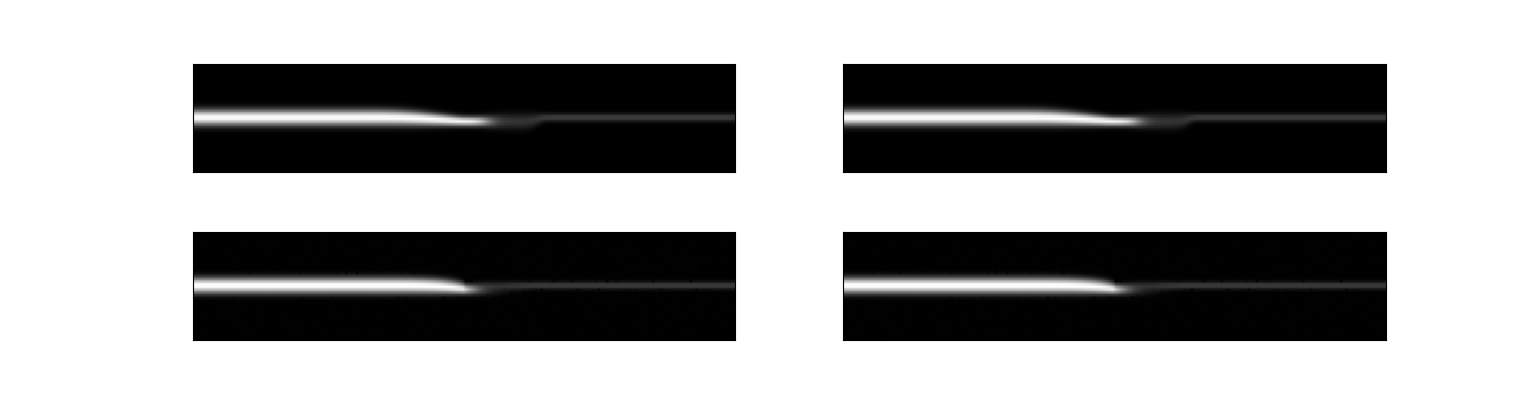
\includegraphics[width=\textwidth, height=0.47\textheight]{figures/B20E1k.png}
			The structure of the velocity space can be recovered after the dimension reduction, but the timely developement is not beeing recognized.
	\end{frame}
	\begin{frame}
		\frametitle{Usin Autoencoders for Reduced Order Modeling}
		\framesubtitle{Results}
		The figure shows the Density at the last timestep of the original data (blue), the SVD data (red dotted) and the recovered data from the autoencoder(green).
		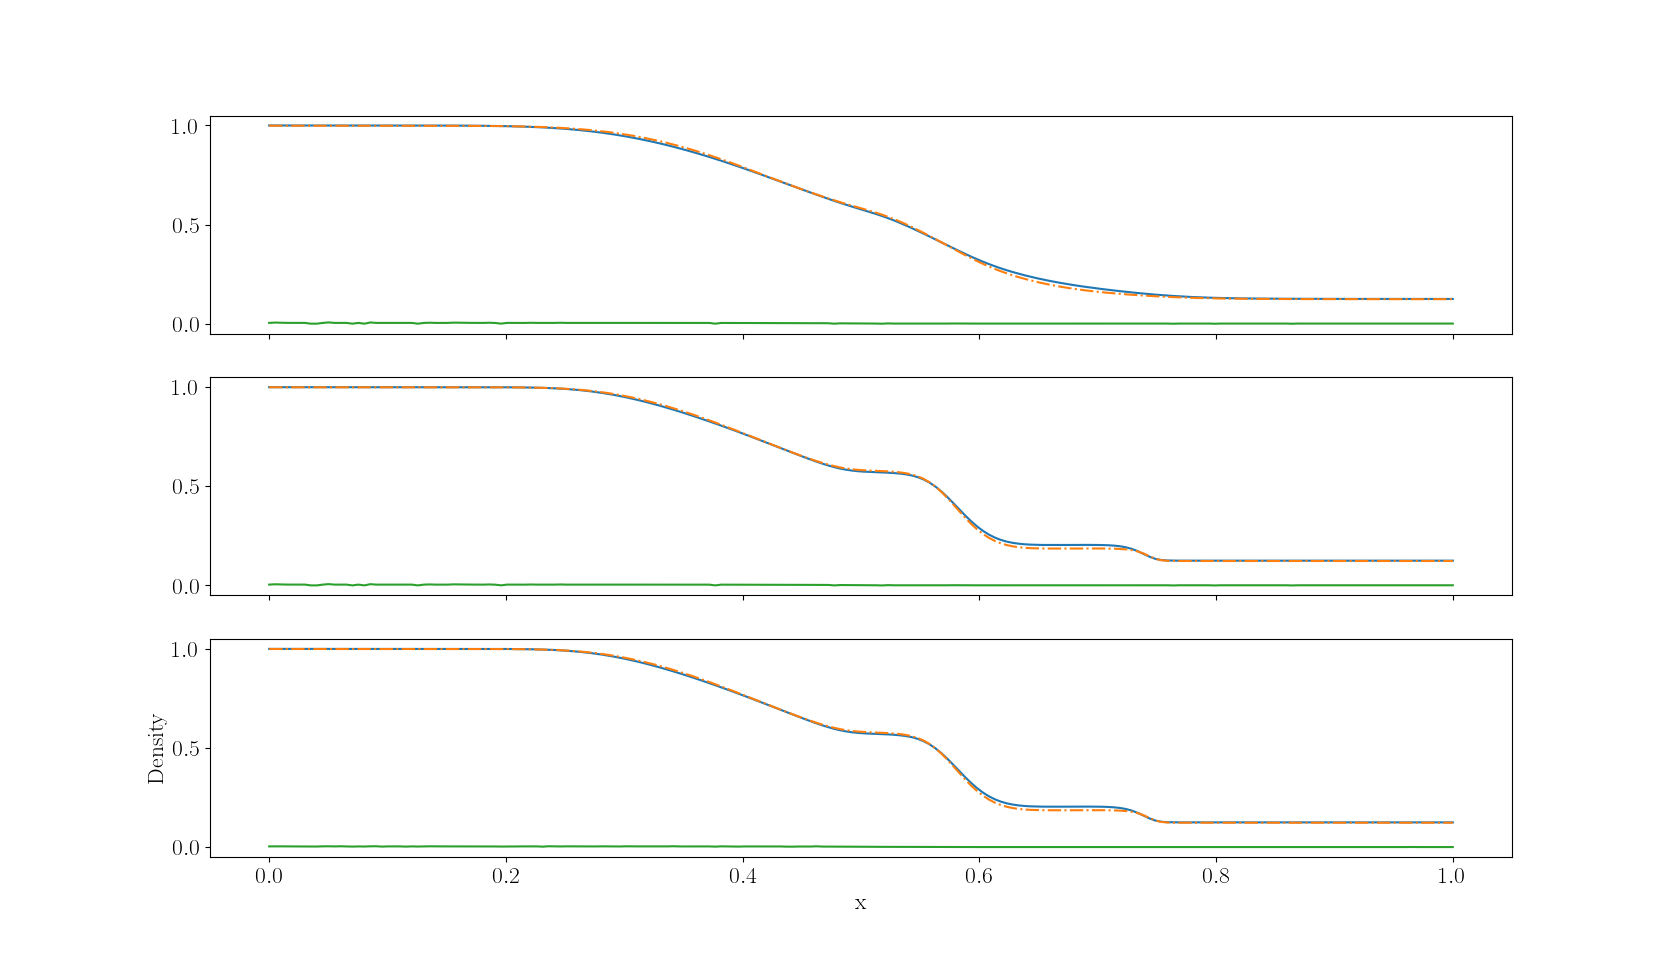
\includegraphics[width=\linewidth]{figures/density.png}
	\end{frame}
	\begin{frame}
		\frametitle{Usin Autoencoders for Reduced Order Modeling}
		\framesubtitle{Literature and Questions}
			Questions and further approches
			\begin{itemize}
				\item Concolutional Autoencoder?, Variational Autoencoder?, Sequence-to-Sequence Autoencoder?
				\item More training data necessary or change of Autoencoder-Architecture sufficent?
			\end{itemize}
			Literature
			\begin{itemize}
			\item Model reduction od dynamical systems on nonlinear manifolds using deep convolutional autoencoders, Kookjin Lee, Kevin T. Carlberg (2019)
			\item Deep Learning, MIT Press book, Goodfellow et al.
			\item ...
			\end{itemize}

	\end{frame}
\end{document}